\chapter{}

\begin{figure}
\centering
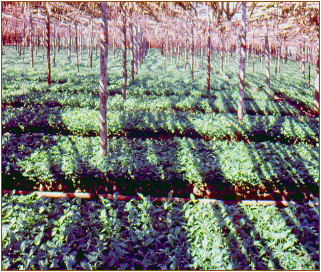
\includegraphics[width=0.8\linewidth]{23/viveiro.png}
\caption{Viveiro de mudas da Santa Teresa.}
\end{figure}

O tempo passava, as mudas vicejavam bonitas no imenso viveiro, as leiras estavam quase secas e Paulo hesitava em tocar fogo na fazenda.
Se não estivessem bem secas, as toras não queimariam direito e cuidar do café na maçaroca seria oneroso e difícil.
Mas, se passasse o dia de queimar, com o tempo das chuvas se aproximando, corríamos o risco de a derrubada brotar e aí seria pior ainda.

Guanayr incentivou:

\textit{``-- Vamos queimar essa noite, Doutor.
Se me autorizar, eu toco fogo para o senhor.'' }

Paulo autorizou.
Noite alta, sob um céu de vidro, frio e estrelado, fomos lá para o rancho dele.
A mulher, docemente solícita, ofereceu-me um banco e uma caneca de chá perfumado de folha de figo.

\textit{``-- Para esquentar e acalmar'', ela disse, ``no seu estado, é bom...
Queimada, para quem não está acostumada, às vezes assusta...'' }

De repente, alguém indicou um ponto à distância, onde pequenas línguas avermelhadas começavam a aparecer buliçosas, de longe em longe.
Depois, entraram a serpentear e crescer, alargar e correr ao longo das divisas, pelo meio das leiras e o vento soprando fez aumentar o que parecia agora, na expressão de um escritor, Monteiro Lobato, creio, \textit{um boitatá monstruoso que ia engolindo tudo}, seus milhares de olhos explodindo em fagulhas, em labaredas que se erguiam para o céu, espalhando um calor de fornalha que já começava a chegar até nós.

Um dia, Chico, um primo do Paulo a quem este incumbiu de comandar os peões numa queimada, descreveu a experiência de se ver no meio de uma como tão alucinante e arrebatadora, que num determinado momento ele quase cedeu à tentação de incrementar aquela celebração do fogaréu, atirando para dentro das chamas tudo o que via pela frente.

A experiência é de fato assustadora porque num certo momento a sensação é de fim de mundo e de que tudo será calcinado.

Ao amanhecer, as chamas foram cedendo, amansando e quando voltamos para o barracão, o que se via era desolação pura: na paisagem cinzenta, tocos enegrecidos apontavam para cima entre os rolos da fumaça que aos poucos se extinguia.
A queimada, na maior parte da fazenda, fora um sucesso.

Pouco tempo depois, teve início o plantio.
Cerca de trinta famílias, em regime de parceria, foram contratadas para formar e cuidar do cafezal.
Eram paranaenses, na sua maior parte.
Fornecemos o material para que construíssem suas casas, de acordo com uma planta simples que a gente mesmo rascunhou.
Em madeira, cobertas de telha.
Cada uma recebeu um pedaço de terra para fazer a roça de subsistência, criar umas galinhas, engordar um porco.
A fazenda virou um pequeno povoado.
Todo dia havia questões a resolver.
Uma briga de vizinhos, uma parturiente ``com o útero virado'', segundo o diagnóstico de Dona Antonia, a parteira, ameaçando entrar em trabalho de parto.
Dormimos de sobreaviso, vestidos, prontos a conduzi-la a Aquidauana assim que os sintomas se apresentassem.
Pela manhã, a moça recebeu-nos sorridente, com o nenê, um meninão de mais de cinco quilos, ao lado.

\textit{``-- Como foi isso?''} perguntei assombrada.

\textit{``- Ah, dona Teresa, não deu tempo de chamar, não.
Deus me ajudou e virei eu mesma, na mão.''} explicou Dona Antonia, toda orgulhosa.
 
Esse seria o primeiro dos muitos milagres que eu testemunharia, forjados pela bárbara medicina dos sertões.

\begin{figure}
\centering
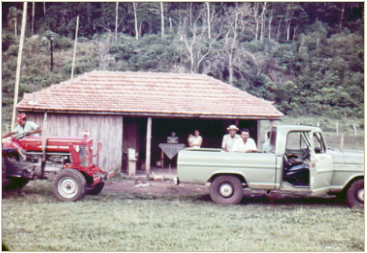
\includegraphics[width=\linewidth]{23/colonos.png}
\caption{Os colonos da Santa Teresa.}
\end{figure}

\begin{figure}
\centering
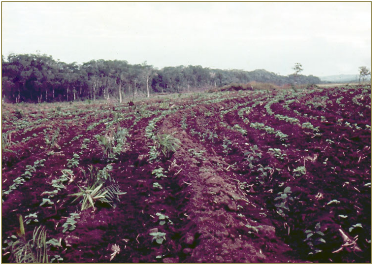
\includegraphics[width=\linewidth]{23/plantio.png}
\caption{O plantio de café.}
\end{figure}

Uma vez na semana, Paulo e eu percorríamos a colônia para anotar os pedidos de coisas a serem providenciadas na cidade.
Remédios, ferramentas, dois metros de pano floridinho -- ``a senhora mesma pode escolher'' --, cartas para pôr no Correio.
Alguns eram engraçados: 

\textit{``-- Dona Rosa, o que é esse chinelo elétrico que a senhora pediu aqui?'' }

\textit{``-- Dona Teresa, ouvi no rádio.
É um chinelo com uma sola que descarrega a energia no chão.
Diz que faz passar o nervoso.
Queria um par para o meu marido, para ele parar de me bater.'' }

Duzentas e cinquenta mil covas de café foram plantadas.
Pouca gente acreditava.
Meu pai, que cresceu em fazenda de café, veio visitar-nos.
Ria, entusiasmado, e exclamava:
\textit{``-Esse cara é louco! Um cafezal desses, nesse fim de mundo? Vai ser corajoso assim no inferno!'' }

Fábio Rodas, amigo do Paulo, agricultor desde o berço, maior plantador individual de laranja do Estado de São Paulo, também custou a crer:
\textit{``-- Preto, você tem muita raça.
Eu não encarava uma empreitada dessas sozinho, nunca!''}.

Mas o cafezal estava lá, bonito, robusto, começando a espalhar seu verde brilhante e profundo pelas terras da fazenda.

\begin{figure}
\centering
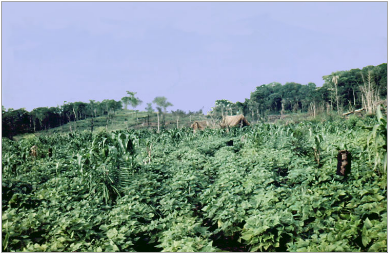
\includegraphics[width=0.8\linewidth]{23/cafezal.png}
\caption{O cafezal da Santa Teresa.}
\end{figure}
  
Enquanto isso, meu menino na barriga crescia também.
Eu já estava pesada e as estradas da Bodoquena, esburacadas pelas chuvas da primavera, tornavam cada viagem um sacrifício e um risco.
Em alguns trechos eu tinha que me ajoelhar sobre o banco da caminhonete para diminuir o desconforto que a trepidação constante provocava.
Deixei de acompanhar o Paulo que começou a ir sozinho para lá.
Viajava na segunda e voltava no sábado.
Durante a semana, eu e o meu bebê vivíamos num universo só nosso, de paz e tranquilidade, preparando-nos para o momento em que ele mostraria sua carinha aqui fora, no mundo.
Com certeza percebendo isso, Paulo não quis me preocupar com as negras nuvens que começavam a pairar sobre o futuro da Santa Teresa.

As denúncias insistentes de que grande parte do café financiado para o Mato Grosso não fora plantado e de que aquele monte de dinheiro tinha sido, na verdade, desviado para outros fins e até levado para fora do país, fez com que o presidente do Instituto Brasileiro do Café decidisse, ele próprio, fazer um sobrevôo sobre a região, para constatar os fatos.
Conta-se que o sujeito desceu do avião à beira de um colapso, indo direto para um pronto-socorro cardiológico.
As denúncias eram quase todas procedentes.
Na Serra da Bodoquena, com exceção do Paulo e de mais três ou quatro cafeicultores, quase ninguém tinha plantado coisa alguma dos milhões de pés financiados para a região.
Alguns sequer tinham chegado até suas terras, como ficava óbvio pela inexistência de estradas ou até de simples picadas que conduzissem até elas.
Outros tinham começado a derrubar e desistido antes de abrir uma cova sequer.
Em poucos dias, Paulo e os outros receberam o aviso de que a liberação das parcelas do financiamento estava suspensa até que uma sindicância apurasse os fatos, separando o joio do trigo.
Estávamos com trinta famílias na colônia e nossa única fonte de recursos era o financiamento.

De início, havia a esperança de que a suspensão seria temporária.
Inebriada com a proximidade do parto, quis acreditar que assim seria e deixei de pensar no assunto.
Nessa época, eu tinha a firme convicção de que Paulo sempre achava um jeito de fazer as coisas darem certo.
Eu havia sido educada na escola pessimista do meu pai, que ensinava a prevenir-se sempre para o pior.
Mas Paulo se irritava com isso, vendo nessa minha postura uma forma de torcer contra suas iniciativas.
Sem querer provocar desgaste naquele momento e admitindo que até então a sorte sorrira para nós, resolvi confiar e pronto.

Decidíramos que era melhor que eu tivesse nosso filho em Araraquara.

Aproximava-se o Natal, a viagem era longa e o médico aconselhou que eu fosse então, de uma vez, e aguardasse o nascimento por lá.